% Template for ICASSP-2010 paper; to be used with:
%          mlspconf.sty  - ICASSP/ICIP LaTeX style file adapted for MLSP, and
%          IEEEbib.bst - IEEE bibliography style file.
% --------------------------------------------------------------------------
\documentclass{article}
\usepackage{amsmath,graphicx,mlspconf}


\copyrightnotice{978-1-4673-7454-5/15/\$31.00 {\copyright}2015 IEEE}

\toappear{2015 IEEE International Workshop on Machine Learning for Signal Processing, Sept.\ 17--20, 2015, Boston, USA}


% Example definitions.
% --------------------
\def\x{{\mathbf x}}
\def\L{{\cal L}}

% Title.
% ------
\title{Filtering of Frequency-Transformed Image 
for Privacy Preserving Facial Recognition}
%
% Single address.
% ---------------
\name{Author(s) Name(s)\thanks{Thanks to XYZ agency for funding.}}
\address{Author Affiliation(s)}
%
% For example:
% ------------
%\address{School\\
%	Department\\
%	Address}
%
% Two addresses (uncomment and modify for two-address case).
% ----------------------------------------------------------
%\twoauthors
%  {A. Author-one, B. Author-two\sthanks{Thanks to XYZ agency for funding.}}
%	{School A-B\\
%	Department A-B\\
%	Address A-B}
%  {C. Author-three, D. Author-four\sthanks{The fourth author performed the work
%	while at ...}}
%	{School C-D\\
%	Department C-D\\
%	Address C-D}
%
\begin{document}
%\ninept
%

\maketitle
%
\begin{abstract}
This paper examines the use of filters on feature vectors for 
privacy protection in facial recognition. Feature vectors are 
the results of Fast Fourier Transform and Wavelet Transform on 
the Yale and Olivetti datasets. Several filters are proposed. 
Filters based on the signal to noise ratio and t test select 
feature which prevent privacy compromising reconstruction without 
sacrificing accuracy. The use of phase removal for FFT and 
normalization are also shown to protect privacy.   
\end{abstract}
%
\begin{keywords}
One, two, three, four, five
\end{keywords}
%
\section{Introduction}
\label{sec:intro}

In modern times, the existence of both terrorist threats and advance digital technology created both the need and the possibility of mass surveillance. A critical competent of such system is biometric identification of people, mainly by facial recognition. As noted in \cite{bowyer2004face}, the events of 9/11, Edward Snowden incident and other events have resulted in both a demand for recognition systems and a concern for privacy violation by such systems. While a lot of research has gone into improving facial recognition systems - \cite{bouzalmat2014comparative}, \cite{spies2000face}, \cite{bouzalmat2011facial}, 
\cite{dehai2013pca}, \cite{samra2003face} among others - relatively little research has been done on incorporating privacy into such systems; some examples being \cite{erkin2009privacy}, \cite{sadeghi2010efficient}, and \cite{kevenaar2005face}.    
\\\\
The primary approach to privacy in facial recognition is cryptography. In \cite{erkin2009privacy}, Eigenfaces recogition system is used on homomorphically encrypted data. In this first cryptographic system for facial recognition \cite{erkin2009privacy}, the client wants the server to identify a face without revealing the image to the server. 
The server also does not want to reveal the contents of it's database. In this approach, data is quantized for Pailler encryption and server and client share computations needed for matching faces. \cite{erkin2009privacy} Experimentally, 96\% accuracy was achieved in \cite{erkin2009privacy} on "ORL Database of Faces". \cite{sadeghi2010efficient} improved the algorithm presented in \cite{erkin2009privacy} by reducing the time and space complexity with the use of garbled circuits. 
\\\\
Along a different line of research, \cite{kevenaar2005face} used Helper Data Systems to provide privacy. The approach generates binary feature vector by determining reliable bits based on statistics from sample data. In the following paper, I investigate a similar approach to privacy. However, in my proposed approach no encryption or quantization is necessary. In my approach there are not additional processes. Privacy is built into the classification process. 
\\\\
This approach rests on the idea that privacy is compromised when an image can be visually inspected by an individual. Therefore, as long as the reconstruction of an image from a feature vector is not meaningful to a human, privacy has been maintained. Facial recognition systems often utilize Fast Fourier Transform (FFT) or Wavelet Transform (WT) as part of feature engineering. For example \cite{spies2000face}, \cite{bouzalmat2011facial}, 
\cite{dehai2013pca}, and \cite{samra2003face} use FFT or WT, their systems can be seen in Figure 1 and 2 and classification accuracies are provided in Figures 3 and 4. I investigate if in recognition systems like these, it is possible to alter the output of FFT or WT to reduce the quality of the reconstructed image without sacrificing accuracy of the classification.           

\section{My Classification Systems}
\label{sec:system}

As picture in Figure 5, my classification systems for this investigation, 
which are very similar, begin with an application of FFT or WT to an image. 
Then a filter is applied as part of feature selection. Classification is 
accomplished with an SVM. For all of the following experiments an SVM with a 
leaner kernel and C = 1 was found to produce the best results.    

\begin{figure}[htb]

\begin{minipage}[b]{1.0\linewidth}
  \centering
  \centerline{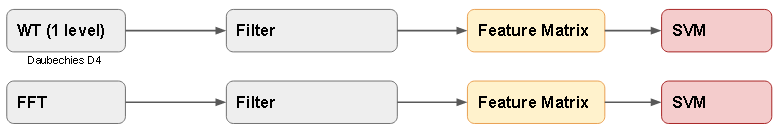
\includegraphics[width=8.5cm]{mysys}}
%  \vspace{2.0cm}
  \centerline{(a) Result 1}\medskip
\end{minipage}
%
\caption{Example of placing a figure with experimental results.}
\label{fig:res}
%
\end{figure}

\section{Filters}
\label{sec:Filters}

A filter is a binary matrix which selects features based on some criteria. 
Let $F_{x,d}$ be a filter $F_{x,d} \in \{0,1\}^{d x m}$ where $m$ is the number of features in each example, $x$ is one of the filter types, and $d$ is the number of features selected by the filter.
\\\\
$F_{x, d,i,j} = 1$ if $W_{x}(j)$ is with in the $d$ largest $W_{x}$, otherwise $F_{d,i,j} = 0$. 
\\\\
Let $X$ be an example: $X_{filtered} =  F_{x,d}X$
\\\\
The following Python code illustrates the mathematical definition above. In this code, 151 examples from X\_nophase are used to compute the variance of each feature, with each feature being the amplitude of a frequency from FFT. Then the 100 features with the highest 
variance are selected to pass thought the filter. 
    
$\\$
Variance is only one of the several filters investigated, and the only unsupervised filter. The other filters include rectangle and triangle filters, inspired by results in \cite{spies2000face}, which are independent of the training data, and 4 supervised filters based on the signal to noise ratio, Fisher discriminant ratio, symmetric divergence and t test. The supervised filters require a labels for positive and negative classes. During training, for each individual the training examples are divided into two classes. Positive class contains the pictures of that individual and the negative class contains all other pictures. The signal to noise ratio, Fisher discriminant ratio, symmetric divergence or t test are computed based on those two classes for each feature, and the final weight for that feature is the mean of weights cross all of the individual in the training set. 
\\\\
The filters are mathematically defined below, expect for the triangle and rectangle filters, for which Python code was a much more succinct form of definition. For the equations below, let $\mu^{+}_{j}$, $\sigma^{+}_{j}$, and $N^{+}_{j}$ be the mean, standard deviation and number of examples for the target person and let $\mu^{-}_{j}$, $\sigma^{-}_{j}$, and $N^{-}_{j}$ be the mean, standard deviation and number of examples for all other people in the database. 

\subsection{Variance}

\begin{equation} \label{Var}
W_{VAR}(j) = \sigma^{2}_{j}
\end{equation}

\subsection{Signal to Noise Ration}

\begin{equation} \label{SNR}
W_{SNR}(j) = \overline{\dfrac{| \mu^{+}_{j} - \mu^{-}_{j} |}{\sigma^{+}_{j} + \sigma^{-}_{j}}}
\end{equation}

\subsection{Fisher Discriminant Ratio}

\begin{equation} \label{FDR}
W_{FDR}(j) = \overline{\dfrac{( \mu^{+}_{j} - \mu^{-}_{j} )^{2}}{(\sigma^{+}_{j})^{2} + (\sigma^{-}_{j})^{2}}}
\end{equation}

\subsection{Symmetric Divergence}

\begin{equation} \label{SD}
W_{SD}(j) = \overline{\dfrac{1}{2} \dfrac{(\mu^{+}_{j})^{2}}{(\mu^{-}_{j})^{2}} + \dfrac{(\mu^{-}_{j})^{2}}{(\mu^{+}_{j})^{2}} + \dfrac{1}{2} \dfrac{( \mu^{+}_{j} - \mu^{-}_{j} )^{2}}{(\sigma^{+}_{j})^{2} + (\sigma^{-}_{j})^{2}} - 1}
\end{equation}

\subsection{T}

\begin{equation} \label{T}
W_{T}(j) = \overline{\dfrac{ \mu^{+}_{j} - \mu^{-}_{j}}{\sqrt{\dfrac{(\sigma^{+}_{j})^{2}}{N^{+}_{j}} + \dfrac{(\sigma^{-}_{j})^{2}}{N^{-}_{j}}}}}
\end{equation}

\subsection{Rectangle}

\begin{figure}[htb]

\begin{minipage}[b]{1.0\linewidth}
  \centering
  \centerline{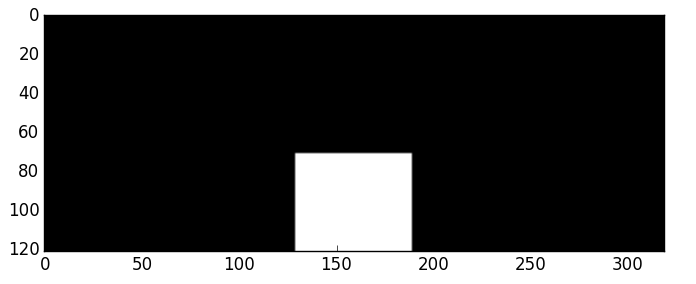
\includegraphics[width=8.5cm]{rect}}
%  \vspace{2.0cm}
  \centerline{(a) Result 1}\medskip
\end{minipage}
%
\caption{Example of placing a figure with experimental results.}
\label{fig:res}
%
\end{figure}

\subsection{Triangle}

\begin{figure}[!htbp]

\begin{minipage}[b]{1.0\linewidth}
  \centering
  \centerline{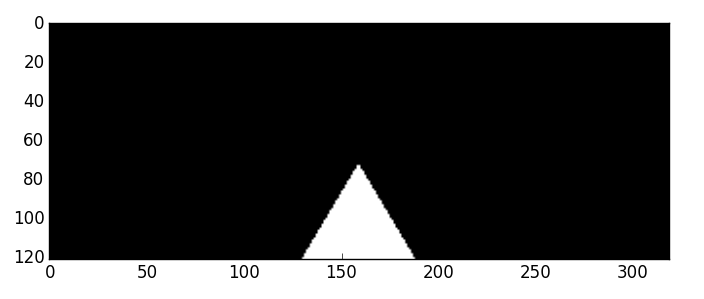
\includegraphics[width=8.5cm]{tri}}
%  \vspace{2.0cm}
  \centerline{(a) Result 1}\medskip
\end{minipage}
%
\caption{Example of placing a figure with experimental results.}
\label{fig:res}
%
\end{figure}

\section{Method}
\label{sec:Method}

\subsection{Classification}

Ten fold cross validation was used to test classification accuracies. Grid Search was used to optimize the SVM parameters for each fold. For all of the following experiments an SVM with a leaner kernel and C = 1 was found to produce the best results. 100 cross validations were performed and the training of supervised and unsupervised filters was constrained to appropriate fold. Since the rectangle and triangle filters are parameterized they were used to determine d for all other filters. For FFT, the filters where only applied to the amplitudes of frequencies. For WT, the filters were applied to all four maps.     

\subsection{Reconstruction}

To reconstruct original images from filtered feature vectors I set the values of all parameters which were filtered out to be zero.  

\section{Experimental Results}
\label{sec:ExperimentalResults}

The baseline accuracy for Yale with FFT transform is 0.741 and 0.735 when the phase is removed. The baseline for Olivetti with FFT transform is 0.975 and 0.9737 with the phase removed. The baseline for Yale with WT transform is 0.807. The baseline for Olivetti with WT transform is 0.963.    

\subsection{Basic Observations}

FFT produces a amplitude and phase for the transformed image. If the phase is removed and the image is reconstructed based on the amplitude the result is a faceless image. The image on the left is of the original, while the image on the right is the reconstruction.   

\begin{figure}[htb]

\begin{minipage}[b]{.48\linewidth}
  \centering
  \centerline{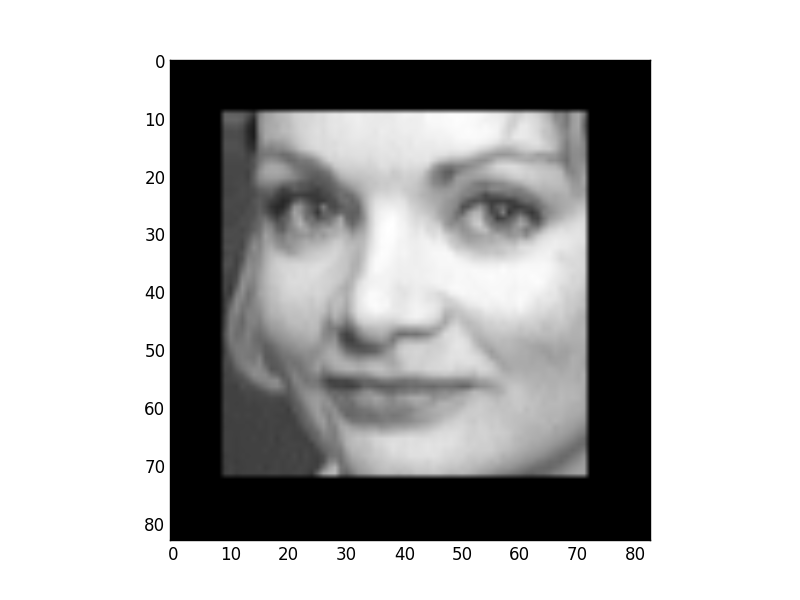
\includegraphics[width=4.0cm]{recon/Original1o}}
%  \vspace{1.5cm}
  \centerline{(b) Results 3}\medskip
\end{minipage}
\hfill
\begin{minipage}[b]{0.48\linewidth}
  \centering
  \centerline{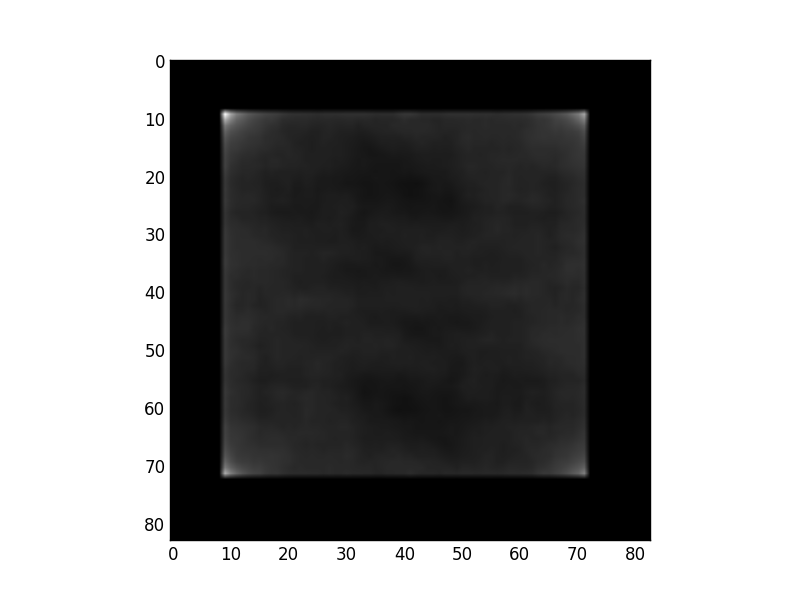
\includegraphics[width=4.0cm]{recon/Recon1o}}
%  \vspace{1.5cm}
  \centerline{(c) Result 4}\medskip
\end{minipage}
%
\caption{Example of placing a figure with experimental results.}
\label{fig:res}
%
\end{figure}

$\\$
A similar phenomena happens when the result of FFT is normalize to zero mean and unit 
variance. Top images are the spectrum and reconstruction of a normalized FFT output. The bottom images show the spectrum and reconstruction for the same image with the original mean and variance restored.    

\begin{figure}[htb]

\begin{minipage}[b]{.48\linewidth}
  \centering
  \centerline{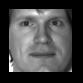
\includegraphics[width=4.0cm]{recon/denorm_Yale}}
%  \vspace{1.5cm}
  \centerline{(Original Image}\medskip
\end{minipage}
\hfill
\begin{minipage}[b]{0.48\linewidth}
  \centering
  \centerline{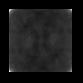
\includegraphics[width=4.0cm]{recon/norm_Yale}}
%  \vspace{1.5cm}
  \centerline{Reconstructed Image}\medskip
\end{minipage}
%
\caption{Example of placing a figure with experimental results.}
\label{fig:res}
%
\end{figure}



\begin{figure}[htb]

\begin{minipage}[b]{.48\linewidth}
  \centering
  \centerline{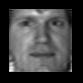
\includegraphics[width=4.0cm]{recon/rectF_399_yale}}
%  \vspace{1.5cm}
  \centerline{Rect 399 0.73}\medskip
\end{minipage}
\hfill
\begin{minipage}[b]{0.48\linewidth}
  \centering
  \centerline{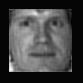
\includegraphics[width=4.0cm]{recon/varF_399_yale}}
%  \vspace{1.5cm}
  \centerline{Var 399 0.739}\medskip
\end{minipage}
%
\begin{minipage}[b]{.48\linewidth}
  \centering
  \centerline{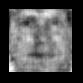
\includegraphics[width=4.0cm]{recon/snrF_399_yale}}
%  \vspace{1.5cm}
  \centerline{SNR 399 0.739}\medskip
\end{minipage}
\hfill
\begin{minipage}[b]{0.48\linewidth}
  \centering
  \centerline{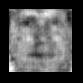
\includegraphics[width=4.0cm]{recon/tF_399_yale}}
%  \vspace{1.5cm}
  \centerline{T 399 0.741}\medskip
\end{minipage}
%
\caption{Example of placing a figure with experimental results.}
\label{fig:res}
%
\end{figure}


\begin{figure}[htb]

\begin{minipage}[b]{.48\linewidth}
  \centering
  \centerline{
\includegraphics[width=4.0cm]{filter/rectF_399}}
%  \vspace{1.5cm}
  \centerline{Rect 399 0.73}\medskip
\end{minipage}
\hfill
\begin{minipage}[b]{0.48\linewidth}
  \centering
  \centerline{
\includegraphics[width=4.0cm]{filter/varF_399}}
%  \vspace{1.5cm}
  \centerline{Var 399 0.739}\medskip
\end{minipage}
%
\begin{minipage}[b]{.48\linewidth}
  \centering
  \centerline{
\includegraphics[width=4.0cm]{filter/snrF_399}}
%  \vspace{1.5cm}
  \centerline{SNR 399 0.739}\medskip
\end{minipage}
\hfill
\begin{minipage}[b]{0.48\linewidth}
  \centering
  \centerline{
\includegraphics[width=4.0cm]{filter/tF_399}}
%  \vspace{1.5cm}
  \centerline{T 399 0.741}\medskip
\end{minipage}
%
\caption{Example of placing a figure with experimental results.}
\label{fig:res}
%
\end{figure}


\begin{figure}[htb]

\begin{minipage}[b]{.48\linewidth}
  \centering
  \centerline{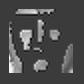
\includegraphics[width=4.0cm]{recon/varF_399_yaleWL}}
%  \vspace{1.5cm}
  \centerline{Var 399 0.737}\medskip
\end{minipage}
\hfill
\begin{minipage}[b]{0.48\linewidth}
  \centering
  \centerline{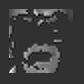
\includegraphics[width=4.0cm]{recon/tF_399_yaleWL}}
%  \vspace{1.5cm}
  \centerline{T 399 0.812}\medskip
\end{minipage}
%
\caption{Example of placing a figure with experimental results.}
\label{fig:res}
%
\end{figure}


\begin{figure}[htb]

\begin{minipage}[b]{1.0\linewidth}
  \centering
    \begin{tabular}{ | l || c | r |}
    \hline
    Filter & Yale Acc & Olliveti Acc \\ \hline
    Rect & 0.737 & 0.967 \\ \hline
    Var & 0.739 & \textbf{0.970} \\ \hline 
    SNR & 0.739 & 0.968 \\ \hline
    FDR & 0.735 & 0.965 \\ \hline
    SD & 0.686 & 0.952 \\ \hline
    T & \textbf{0.741} & 0.968 \\
    \hline
    \end{tabular}
  \centerline{(a) Result 1}\medskip
\end{minipage}
%
\caption{Mean accuracy for the filters based on 100, 10 fold cross validations. Top 399 features are
selected for a total feature vector of 2415.}
\label{fig:res}
%
\end{figure}



\begin{figure}[htb]

\begin{minipage}[b]{1.0\linewidth}
  \centering
    \begin{tabular}{ | l || c | r |}
    \hline
    Filter & Yale Acc & Olliveti Acc \\ \hline
    Var & 0.737 & 0.941 \\ \hline 
    SNR & \textbf{0.813} & 0.968 \\ \hline
    FDR & 0.807 & \textbf{0.969} \\ \hline
    SD & 0.672 & 0.883 \\ \hline
    T & 0.812 & \textbf{0.969} \\
    \hline
    \end{tabular}
  \centerline{(a) Result 1}\medskip
\end{minipage}
%
\caption{Mean accuracy for the filters based on 100, 10 fold cross validations. Top 399 features are
selected for a total feature vector of 2415.}
\label{fig:res}
%
\end{figure}


% To start a new column (but not a new page) and help balance the last-page
% column length use \vfill\pagebreak.
% -------------------------------------------------------------------------
\vfill
\pagebreak

\section{Conclusions}
\label{sec:conclusion}
$\\$
There is a lot of potential for privacy protection with proper alterations in the feature engineering process. Across all experiments the removal of the phase from the FFT result yields almost the same accuracy. However, the image becomes impossible reconstruct using simple means. Additionally, the normalization mean and variance can be hidden by the server, which also prevents reconstruction. Along the same lines, the feature vectors can be permuted by some hidden permutation matrix. 
\\\\
Regarding the filters, which should be applied even for performance improvements, SNR and T are the most useful for privacy protection. For both FFT and WT, these filters allow a large dimension reduction with almost no accuracy loss. This allows for reconstructions to be unidentifiable, see Table 11 cells j and v and Table 13 cells f and r. In general the supervised filter promote privacy in the reconstructed image. This is because they use high and low frequencies for reconstruction in FFT as seen in Table 12. The mix avoid details form being reconstructed fully. In WT, the filters prevent reconstruction of the eyes which is useful, although not fully understood. For high level of privacy, rectangle, triangle and variance filter performs best across experiments at the smallest tried d. 
\\\\
In future research consecutive search methods can be utilized to produce filters. Additionally, the reconstruction for WT should be explained in terms of the underlying bands. Lastly, a fully algorithm utilizing the filters and taking into the account the client server model should be developed.  
\\\\\\\\
This paper represents my own work in accordance with University regulations.              
\\\\\\\\

\section{REFERENCES}
\label{sec:ref}

List and number all bibliographical references at the end of the paper.  The references can be numbered in alphabetic order or in order of appearance in the document.  When referring to them in the text, type the corresponding reference number in square brackets as shown at the end of this sentence \cite{bouzalmat2014comparative}.

% References should be produced using the bibtex program from suitable
% BiBTeX files (here: strings, refs, manuals). The IEEEbib.bst bibliography
% style file from IEEE produces unsorted bibliography list.
% -------------------------------------------------------------------------
\bibliographystyle{IEEEbib}
\bibliography{sources} 

\end{document}
